\section{Maschienenbau (Simbürger)}

\subsection{Planung}

\subsubsection{Rahmen}

\subsubsection{X-Achse}

\paragraph{Antrieb}

\paragraph{Schlittenauslegung}

\paragraph{Kabelführung}

\subsubsection{Y-Achse}
\paragraph{Motorauslegung}

\subsubsection{Z-Achse ("Gabel")}
\paragraph{Positionsbestimmung}

\subsection{Ferttigung}

\paragraph{Umlenkrollen}
Die Umlenkrollen sind jeweils am Ende der X- und Y-Achsen angebracht. Dadurch dass diese der gesamten Spannkraft ausgesetzt. Dies erfordert spezielle Anforderungen an die Aufhängen als auch an die Umlenkrolle selbst. Diese soll primär eine 180° Wende des Zahnriemens ermöglichen, sowie sekundär eine Führung für den Riemen bieten. 
Umgesetzt wird diese Anforderungen, durch Fertigung von vier Aluminium-Drehteilen in welche Kugellager eingepresst werden.

\begin{figure}[h]
    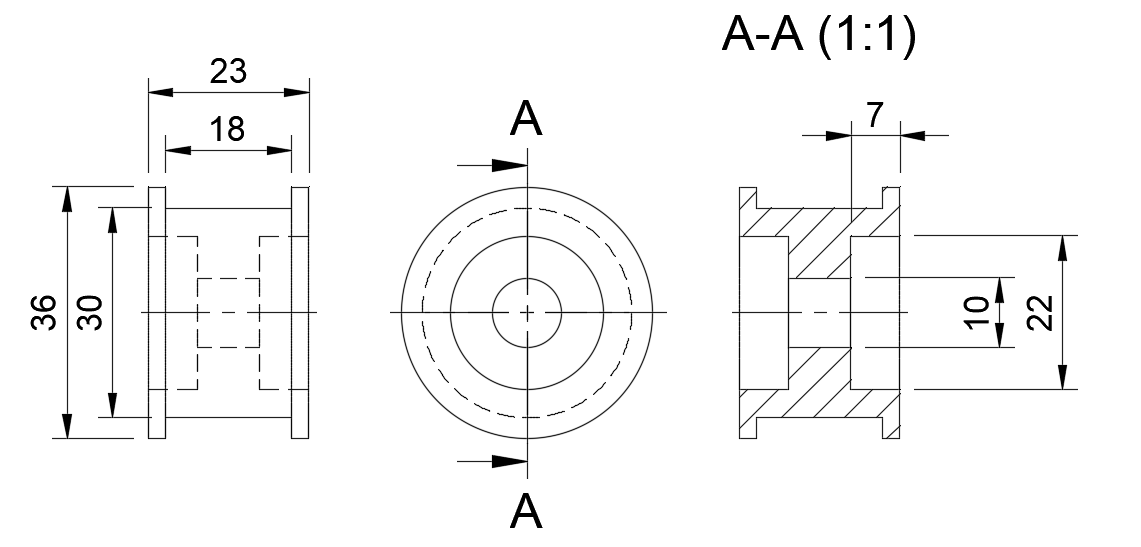
\includegraphics[width=0.5\textwidth]{AT5x16-Umlenkung.png}
    \centering
    \caption{Bauteilzeichnung Umlenkrolle}
\end{figure}

Die Fertigung dieses Teils Lässt sich in folgende Teilschritte unterteilen:
\begin{itemize}
    \setlength\itemsep{0mm}
    \item Zuerst die Frontfläche Plandrehen (900U/min)
    \item Ungefär 30mm Länge auf das Aussenmaß von 36mm Plandrehen
    \item Mit 9.8mm Bohrer das mittlere Loch vorbohren (540U/min)
    \item Mit 10mm Reibeisen und viel Öl das Loch auf eine genaue passung bringen (260U/min)
    \item Die Position Relativ zum Backenfutter makieren um beim neu einspannen Rundlaufgenauigkeit gewährzuleisten
    \item Zylinder bei ca. 26 mm Abstechen (540U/min)
    \item Umspannen und auf maß plandrehen (900U/min)
    \item Die Aussparung für die Lager mit Eckdrehmeissel beginnen, jedoch nach innen hin nur 6.8 mm 
    \item Bei ca. 17 mm Lochdurchmesser den tatsächleichen Durchmesser mit der Digitalanzeige vergleichen und gegebenennfalls korrigieren
    \item Bei 21.5 mm den Oberschlitten die restlichen 0.2 mm zustellen und die gesamte Tiefe plandrehen
    \item Den Lochdurchmesser auf 21.95 erweitern, und dann in kleinen inkrementen zustellen bis das Lager gerade so nicht passt, um einen Pressitz zu gewährleisten, dies tritt mit 22 mm OD Lagern bei rund 22.04 mm ein
\end{itemize}

    Durch die Verhältnissmäßig großen Toleranzen bei den Lageraussendurchmessern wird bei 2 der 8 Lagerpassungen zusätztlich Lagerkleber verwendet um eine Zuverlässige Passung zu gewährleisten.

    Da für die Einsparung der Riemenführungsfläche kein Angriffspunkt verfühbar ist 


\subsection{Konstruktion}

\section{Software (Simbürger)}
